\section{Implementation and Evaluation}
\label{sec:imp}
The algorithm presented in the last section is idealized.
For example, the semantics of the {\tt parse\_all} function does not
exactly corresponds to the semantics of union and array parsing in \pads 
\cite{fisher+:popl06}. The algorithm is also not optimized.
Parsing unions and arrays both cause the number of parses to 
grow exponentially. Furthermore, the number of aggregates is of 
$O(m ^ n)$, where $m$ is the largest
number of parses for a given data line, and $n$ is the number of lines to aggregate.
Computing at these scales is certainly not practical.
Next, we will discuss some implementation issues in three areas: the correctness of the
learned description, the quality of the learned description and the performance of
the system. And at the end, we will present some preliminary experimental results.

\subsection{Correctness}
\pads{} implements deterministic unions. In other words, the \pads~ parser
only attempts the second branch if the first branch fails to parse. As
such, in the implementation of the incremental learning system, when parsing
$d_1 + d_2$, we first parse $d_1$, and attempt $d_2$ only if there is no
successful parse in the result of parsing $d_1$. This ensures that
updated description, when translated to \pads{} is correct. 
\pads{} also has a ``longest-match'' array semantics, which means when parsing
an array, it repeatedly parsing the body of the array until no progress can be made 
in the input. We adopt a similar strategy in our implementation.
The above two strategies reduces the number of parses to be produced and 
effectively improves the efficiency of the system. 

\subsection{Quality}
In the algorithm presented in section \ref{sec:algo}, parsing a sync token results
in one of three modes: {\tt Good}, {\tt Fail} and {\tt Recovered}. 
In the implementation, a sync token can be not only a constant string, but also
a constant integer, an integer range or an enumeration of the above.
Consider the following scenario. 
The sync token we want to parse is {\tt Sync (Str "GET")},
and the prefix of the current input string is ``POST''. According to the
definition of {\tt parse\_base} function, the result would be {\tt Fail}.
In reality, the input ``POST'' is in the same {\em class} as ``GET'', 
i.e. an English word,
and it may very well be the case that this sync token should have been 
an an enumerations of words, instead of a constant word.
To handle such cases, we created a fourth mode, {\tt Partial} to indicate that. 
the input contains some data that has the same class as the description,
but there is no exact match. During aggregation, such partial nodes in the parse
tree will be noted and treated specially. In the above example, the aggregate 
function will change the description to {\tt sync (Enum [Word "Get", Word "POST"])}.
The introduction of partial nodes can avoid a lot of unnecessary parsing errors
and produce a description that is more compact and meaningful. 

However, there is an issue which could undermine the benefits of partial nodes.
We mentioned earlier that our initial description can be obtained by learning
from an initial chunk of data using the \learnpads{} algorithm. In addition,
the {\tt update\_desc} function uses the \learnpads{} algorithm to learn 
sub-descriptions from all the accumulated data at the various learn nodes 
in the aggregate structure. One of the rewriting rules used in \learnpads{}
merges adjacent constant strings together into one string. As a result, we
could end up with constant strings like ``$\backslash$"GET '' 
(see Fig \ref{fig:ai.p}), instead of ``$\backslash$"'', ``GET'' and `` ''. 
Once multiple words are
concatenated together, it is difficult to categorize its class, or to
produce a partial node based on the class. We therefore delay the application of
this rewriting rule until the every end of the entire incremental learning process.

Another related issue concerns the introduction of {\tt Recovered} nodes 
during parsing. We implement a heuristics that if a sync token is recovered
after skipped too many characters (as a factor of the number of characters in
the sync token itself), we also introduce a {\tt Fail} parse for this sync
token as if this sync token cannot parse at all, and then continue parsing the 
remaining descriptions. This heuristics delayed a decision to commit to
either the recovery or failure. Such decision will be made by comparing the 
``goodness'' of the different parses which will be discussed in the next
subsection.

Finally, when the current description of an incremental step is being updated
using the aggregate, a number of rewriting rules are applied to the new
description to improve its quality and readability. Most of the rules are
data-independent, such as flattening of nested structs and unions, factoring
of structures and removing degenerated lists, which are also used in the 
\learnpads{} system. One unique {\em data dependent} rule used here
is {\em MergeOpts}. Because the aggregate function
introduces opt nodes above a base or sync node in the aggregate structure
whenever the corresponding base or sync token in the description failed to 
parse. This algorithm may introduce a series of opt nodes if the data we
are learning has never been described before and therefore incurring many
failures. The MergeOpts rule collapses the consecutive opt nodes in a 
description if there is a correlation among the branching decisions made
at each of the opt nodes. To do that, we maintain an OptsTable that records
these branching decisions when parsing each data line, and then use the
this table to determine if and how to merge the adjacent opt nodes during
rewrite. The effect of this rule is illustrated in 
Figure \ref{fig:opts} in which
$S$ denotes a struct, and $B$ denotes a base token.

\begin{figure}[t]
\begin{center}
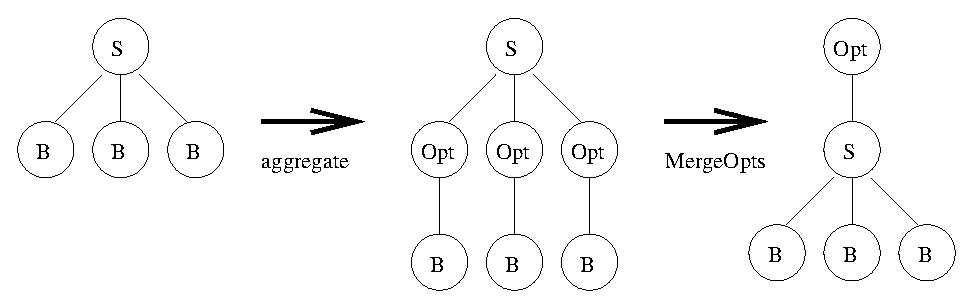
\epsfig{file=opts.eps,width=\columnwidth}
\caption{MergeOpts rewriting rule}\label{fig:opts}
\end{center}
\end{figure}


\subsection{Performance}
Several optimizations have been implemented to contain the number of
parses and aggregates. First, instead of returning all the possible
parses when parseing a description component $d$, 
we rank the parses by a metric, which
measures the ``quality'' of the parse and only return the top $k$
parses. The metric is a triple:
\[m = (e,~ s,~ c)\]
where $e$ is the number of errors, $s$ is the number of skipped
characters during sync token recovery, and $c$ is the number
of characters correctly parsed. A metric is considered ``perfect'', if $e = 0$.
$m_1$ is better than $m_2$ if $m_1$ is perfect and $m_2$ is not, or
if 
\[\frac{c_1}{s_1+c_1} > \frac{c_2}{s_2 + c_2}.\]

In practice, {\tt parse\_all} returns a list of
{\em parse triples} $(r,~m,~j)$, where $r$ is the data representation of
the parse, $m$ is the metric associated with $r$, and
$j$ is the current position of the input after the parse.
We define a {\tt clean} function that does the following.
It takes as input the list of {\em parse triples}, and group
them according to the {\em span} of the parse. The span is
the substring in the input consumed by the parse,
and is marked by a begin and an end position.
Then for each group, it sorts the parse triples by
their metric and retains only the perfect parses and if there
is no perfect parse, the best parse in the group. 
The justification for throwing away all the other parse triples
is that given a description $d$, and a fixed span, we always
prefer the parse with strictly better metric. This idea is
similar to the techniques used in Earley Parsers \cite{earley-parser}, 
though the latter use a chart. Finally {\tt clean} returns all
the perfect triples plus up to top $k$ non-perfect triples.
The {\tt clean} function, when applied to the list of triples
returned by {\tt parse\_all},  reduces the number of bad parses 
to a constant $k$, while guaranteeing that if there is at least one
perfect parse, it will be returned. 

Not only do we clean the list of parses by throwing away
unpromising parses, we also end the parsing of a description
prematurely using a technique called {\em parse cut-off}.
When parsing a struct of multiple
fields, $f_1$, $f_2$, ..., $f_n$, if the algorithm encounters 
a certain number of errors, say 3, in succession, it cancels the
parsing of this struct and returns an empty list. However,
this technique may end up returning empty list for
the entire description. When this happens, we re-parse the whole
description with parse cut-off feature turned off. 

Another important optimization is the memoization.
The program keeps a global memo table indexed by a pair:
description $d$ and the begin position for parsing $d$.
The result for parsing $d$ at the specific position
will be saved and reused. 

Finally, we set an upper limit to the number of aggregates the
algorithm can produce at any point in time by selecting the top
$k$ aggregates with fewest number of opt and learn nodes.
In the next subsection, we will show the effectiveness 
of some of these optimizations.

\subsection{Experiments}
\begin{table}[th]
\begin{tabular}{|c|c|c|c|c|c|}\hline
& & \multicolumn{2}{|c|}{\learnpads} & \multicolumn{2}{|c|}{incremental} \\ \cline{3-6}
\raisebox{1.5ex}[0pt]{Formats} & \raisebox{1.5ex}[0pt]{Lines} &
	Time & CT & Time & CT \\ \hline \hline
ai.3000	&	3000	& 27.5	& 412.6	& 2.1	& 571.0	\\ \hline
asl.log  &	1500	& 31.9	& 960.1	& 23.9 	& 1393.3 \\ \hline
apache.txt  &	2087	& 104.2 & 6111.4& 6.6 	& 2339.5 \\ \hline
access\_log  &	8188 	& 134.5	& 351.2	& 2.9	& 321.2	\\ \hline
error\_log  &	4510	& 101.7	& 101.9	& 0.9	& 107.9 \\ \hline
interface.loop & 1253	& 54.0	& 741.4	& 1.9	& 1053.7 \\ \hline
\end{tabular}
\caption{Execution times (secs) and type complexity (bits)} 
\label{tab:results}
\end{table}


% - parse metric
% - initial learn size and chunk size - these can affect results
% - update chunk by chunk 
% - optimizations/heuristics
%   due to performance concerns:
%   - memoization
%   - the clean function (to reduce the number of parses)
%   - control of aggregate size
%   - parses cut-off: kill a parse if it has more than n consecutive failures in a struct
%   due to quality of description concerns (and also performance)
%   - deterministic unions
%   - longest match in arrays
%   - merge adjacent const strings (only punctuation and white spaces)
%   - error recovery
%
%- Experiments
%	1) comparison with old LearnPADS on several large datasets (ai.3000, asl.log, apache.txt, access\_log, error\_log, interface.loop)
%	   compare exec time and type complexity. For increment, use
%	   initial learn chunk of 100 and incremental error chunks of 100
%	2) use ai format, do a table with 1000 5000 10000,...,1M miles
%	   using orig learning system and the new system with various optimization turned on and off.
%

